\documentclass[journal,12pt,twocolumn]{IEEEtran}

\usepackage{setspace}
\usepackage{gensymb}
\singlespacing
\usepackage[cmex10]{amsmath}

\usepackage{amsthm}

\usepackage{mathrsfs}
\usepackage{txfonts}
\usepackage{stfloats}
\usepackage{bm}
\usepackage{cite}
\usepackage{cases}
\usepackage{subfig}

\usepackage{longtable}
\usepackage{multirow}

\usepackage{enumitem}
\usepackage{mathtools}
\usepackage{steinmetz}
\usepackage{tikz}
\usepackage{circuitikz}
\usepackage{verbatim}
\usepackage{tfrupee}
\usepackage[breaklinks=true]{hyperref}
\usepackage{graphicx}
\usepackage{tkz-euclide}

\usetikzlibrary{calc,math}
\usepackage{listings}
    \usepackage{color}                                            %%
    \usepackage{array}                                            %%
    \usepackage{longtable}                                        %%
    \usepackage{calc}                                             %%
    \usepackage{multirow}                                         %%
    \usepackage{hhline}                                           %%
    \usepackage{ifthen}                                           %%
    \usepackage{lscape}     
\usepackage{multicol}
\usepackage{chngcntr}

\DeclareMathOperator*{\Res}{Res}
\newtheorem{theorem}{Theorem}[section]
\newtheorem{corollary}{Corollary}[theorem]
\newtheorem{lemma}[theorem]{Lemma}
\newtheorem{definition}{Definition}[section]
\renewcommand\thesection{\arabic{section}}
\renewcommand\thesubsection{\thesection.\arabic{subsection}}
\renewcommand\thesubsubsection{\thesubsection.\arabic{subsubsection}}

\renewcommand\thesectiondis{\arabic{section}}
\renewcommand\thesubsectiondis{\thesectiondis.\arabic{subsection}}
\renewcommand\thesubsubsectiondis{\thesubsectiondis.\arabic{subsubsection}}


\hyphenation{op-tical net-works semi-conduc-tor}
\def\inputGnumericTable{}                                 %%

\lstset{
%language=C,
frame=single, 
breaklines=true,
columns=fullflexible
}
\begin{document}

\newcommand{\BEQA}{\begin{eqnarray}}
\newcommand{\EEQA}{\end{eqnarray}}
\newcommand{\define}{\stackrel{\triangle}{=}}
\bibliographystyle{IEEEtran}
\raggedbottom
\setlength{\parindent}{0pt}
\providecommand{\mbf}{\mathbf}
\providecommand{\pr}[1]{\ensuremath{\Pr\left(#1\right)}}
\providecommand{\qfunc}[1]{\ensuremath{Q\left(#1\right)}}
\providecommand{\sbrak}[1]{\ensuremath{{}\left[#1\right]}}
\providecommand{\lsbrak}[1]{\ensuremath{{}\left[#1\right.}}
\providecommand{\rsbrak}[1]{\ensuremath{{}\left.#1\right]}}
\providecommand{\brak}[1]{\ensuremath{\left(#1\right)}}
\providecommand{\lbrak}[1]{\ensuremath{\left(#1\right.}}
\providecommand{\rbrak}[1]{\ensuremath{\left.#1\right)}}
\providecommand{\cbrak}[1]{\ensuremath{\left\{#1\right\}}}
\providecommand{\lcbrak}[1]{\ensuremath{\left\{#1\right.}}
\providecommand{\rcbrak}[1]{\ensuremath{\left.#1\right\}}}
\theoremstyle{remark}
\newtheorem{rem}{Remark}
\newtheorem*{remark}{Remark}
\newcommand{\sgn}{\mathop{\mathrm{sgn}}}
\providecommand{\abs}[1]{\vert#1\vert}
\providecommand{\res}[1]{\Res\displaylimits_{#1}} 
\providecommand{\norm}[1]{\lVert#1\rVert}
%\providecommand{\norm}[1]{\lVert#1\rVert}
\providecommand{\mtx}[1]{\mathbf{#1}}
\providecommand{\mean}[1]{E[ #1 ]}
\providecommand{\fourier}{\overset{\mathcal{F}}{ \rightleftharpoons}}
%\providecommand{\hilbert}{\overset{\mathcal{H}}{ \rightleftharpoons}}
\providecommand{\system}{\overset{\mathcal{H}}{ \longleftrightarrow}}
	%\newcommand{\solution}[2]{\textbf{Solution:}{#1}}
\newcommand{\solution}{\noindent \textbf{Solution: }}
\newcommand{\cosec}{\,\text{cosec}\,}
\providecommand{\dec}[2]{\ensuremath{\overset{#1}{\underset{#2}{\gtrless}}}}
\newcommand{\myvec}[1]{\ensuremath{\begin{pmatrix}#1\end{pmatrix}}}
\newcommand{\mydet}[1]{\ensuremath{\begin{vmatrix}#1\end{vmatrix}}}
\numberwithin{equation}{subsection}
\makeatletter
\@addtoreset{figure}{problem}
\makeatother
\let\StandardTheFigure\thefigure
\let\vec\mathbf
\renewcommand{\thefigure}{\theproblem}
\def\putbox#1#2#3{\makebox[0in][l]{\makebox[#1][l]{}\raisebox{\baselineskip}[0in][0in]{\raisebox{#2}[0in][0in]{#3}}}}
     \def\rightbox#1{\makebox[0in][r]{#1}}
     \def\centbox#1{\makebox[0in]{#1}}
     \def\topbox#1{\raisebox{-\baselineskip}[0in][0in]{#1}}
     \def\midbox#1{\raisebox{-0.5\baselineskip}[0in][0in]{#1}}
\vspace{3cm}
\title{Quiz 2}
\author{Yashas Tadikamalla - AI20BTECH11027}
\maketitle
\newpage
\bigskip
\renewcommand{\thefigure}{\theenumi}
\renewcommand{\thetable}{\theenumi}
Download all python codes from 
\begin{lstlisting}
https://github.com/YashasTadikamalla/EE3900/blob/main/Quiz2/codes
\end{lstlisting}
%
and latex-tikz codes from 
%
\begin{lstlisting}
https://github.com/YashasTadikamalla/EE3900/blob/main/Quiz2/Quiz2.tex
\end{lstlisting}
\section{Problem 3.25}
Consider a right-sided sequence $x[n]$ with $z$-transform 
$$X(z)=\dfrac{1}{\brak{1-az^{-1}}\brak{1-bz^{-1}}}=\dfrac{z^2}{\brak{z-a}\brak{z-b}}$$
In section 3.3 we considered the determination of $x[n]$ by carrying out a partial fraction expansion, with $X(z)$ considered as a ratio of polynomials in $z^{-1}$. Carry out a partial fraction expansion of $X(z)$, considered as a ratio of polynomials in $z$, and determine $x[n]$ from this expansion.
\section{Solution}
\begin{definition}[Z-transform]
The $z$-transform of a discrete time signal $x[n]$ is defined as
\begin{align}
    X(Z)=\displaystyle\sum_{n=-\infty}^{\infty}x[n]z^{-n}
\end{align}
\end{definition}
\begin{remark}
The inverse $z$-transform of $X(Z)$ is $x[n]$
\end{remark}
\begin{definition}[Poles and zeroes of Z-transform]
The values of $z$ for which $X(z)$ is zero are called zeroes, while the values of $z$ for which $X(z)$ is infinite, are called poles.
\end{definition}
\begin{definition}[ROC]
The region of convergence (ROC) is the set of values of z for which $z$-transform converges.
\end{definition}
\begin{remark}
For a right-sided sequence, the ROC extends outward from the outermost finite pole of $X(z)$ to $z=\infty$
\end{remark}
\begin{lemma}
$z$-tranform of $x[n]=\delta[n]$ is $X(z)=1,ROC:\forall z$
\end{lemma}
\begin{proof}
\begin{align}
 X(z)&=\displaystyle\sum_{n=-\infty}^{\infty}\delta[n]z^{-n}\\
    X(z)&=z^{0}=1
\end{align}
As it is defined $\forall z, ROC: \forall z$
\end{proof}
\begin{corollary}
    Inverse $z$-transform of $X(z)=1,ROC:\forall z$ is $x[n]=\delta[n]$
    \label{eq:1}
\end{corollary}
\begin{lemma}
$z$-transform of $x[n]=a^{n-k}u[n-k]$ is $X(z)=\dfrac{z^{-k}}{1-az^{-1}},ROC:\abs{z}>\abs{a}$
\end{lemma}
\begin{proof}
\begin{align}
    x[n]&=a^{n-k}u[n-k]\\
    \Rightarrow X(z)&=\displaystyle\sum_{n=-\infty}^{\infty}a^{n-k}u[n-k]z^{-n}\\
    &=\displaystyle\sum_{n=k}^{\infty}a^{n-k}z^{-n}=a^{-k}\displaystyle\sum_{n=k}^{\infty}a^{n}z^{-n}
\end{align}
If $\abs{az^{-1}}<1$, 
\begin{align}
    X(z)&=a^{-k}\dfrac{a^kz^k}{1-az^{-1}},ROC:\abs{z}>\abs{a}\\
    &=\dfrac{z^{-k}}{1-az^{-1}},ROC:\abs{z}>\abs{a}
\end{align}
\end{proof}
\begin{corollary}
    Inverse $z$-transform of $X(z)=\dfrac{z^{1-k}}{z-a},ROC:\abs{z}>\abs{a}$ is $x[n]=a^{n-k}u[n-k]$
    \label{eq:2}
\end{corollary}

Given, a right-sided sequence $x[n]$ with $z$-transform 
\begin{align}
   X(z)&=\dfrac{1}{\brak{1-az^{-1}}\brak{1-bz^{-1}}}\\
   &=\dfrac{z^2}{\brak{z-a}\brak{z-b}} 
\end{align}
Clearly, $X(n)$ has two zeroes at $z=0$ and $z=a$,$z=b$ are the poles. Without loss of generality, let $z=a$ be the outermost pole. Then, the ROC is $\abs{z}>\abs{a}$ .


Adding and subtracting 1 in RHS
\begin{align}
    X(z)&=1+\dfrac{z^2}{\brak{z-a}\brak{z-b}} -1\\
    &=1+\dfrac{z(a+b)-ab}{\brak{z-a}\brak{z-b}}
\end{align}
Multiplying and dividing with $(a-b)$
\begin{align}
    X(z)&=1+\dfrac{a^2(z-b)-b^2(z-a)}{\brak{z-a}\brak{z-b}\brak{a-b}}\\
    &=1+\dfrac{1}{a-b}\brak{\dfrac{a^2}{z-a}-\dfrac{b^2}{z-b}}\\
    &=1+\dfrac{a^2}{a-b}\brak{\dfrac{1}{z-a}}-\dfrac{b^2}{a-b}\brak{\dfrac{1}{z-b}}
\end{align}
Using \eqref{eq:1},\eqref{eq:2} for $(k=1)$,
\begin{align}
    x[n]&=\delta[n]+\dfrac{a^2}{a-b}a^{n-1}u[n-1]-\dfrac{b^2}{a-b}b^{n-1}u[n-1]\\
    \therefore x[n]&=\delta[n]+\dfrac{a^{n+1}}{a-b}u[n-1]-\dfrac{b^{n+1}}{a-b}u[n-1]
\end{align}
\begin{figure}[!h]
 \centering
 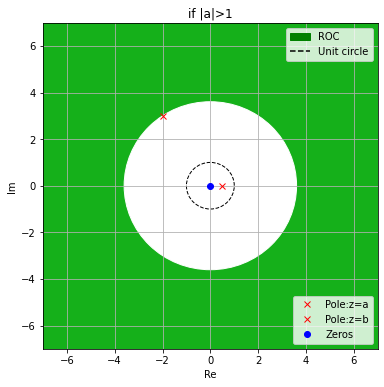
\includegraphics[width=\columnwidth]{Quiz2(1).png}
 \caption{A possible pole-zero plot with $ROC$}
 \label{plot}
\end{figure}
\begin{figure}[!h]
 \centering
 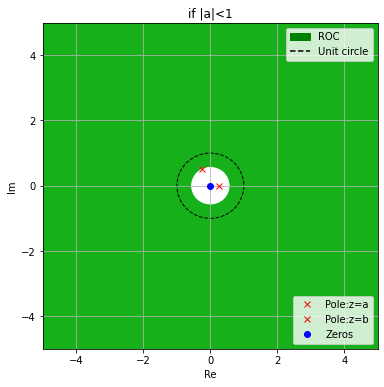
\includegraphics[width=\columnwidth]{Quiz2(2).png}
 \caption{A possible pole-zero plot with $ROC$}
 \label{plot}
\end{figure}
\end{document}


